\chapter{Appendix}

\section{Discussion of the Reduced System Definition}
\label{sec:redsysdef}
The subtleties of the reduced system definition can be better understood with an example.  Consider two 2-level systems and a single particle shared between them (e.g.\ a single electron in a double quantum dot where each dot only contains two energy levels).  This system can be seen schematically in Fig.\ \ref{fig:ddqd}
\begin{figure}[th]
\centering
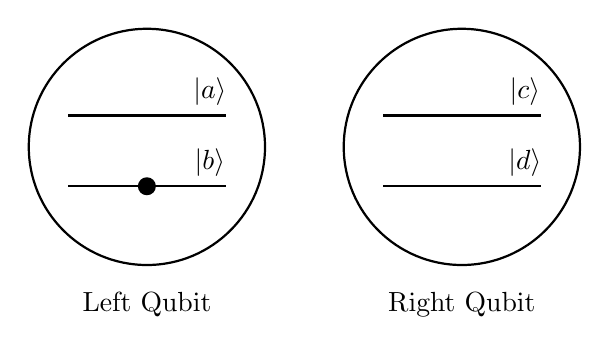
\begin{tikzpicture}
\draw [thick] (3,0.5) circle [radius=1.5];
\draw [thick] (7,0.5) circle [radius=1.5];
\draw [thick] (2.0,0.9) -- (4.0,0.9);
\draw [thick] (2.0,0.0) -- (4.0,0.0);
\draw [thick] (6.0,0.9) -- (8.0,0.9);
\draw [thick] (6.0,0.0) -- (8.0,0.0);
\draw [fill,thick] (3,0.0) circle [radius=0.1];
\node at (3,-1.5) {Left Qubit};
\node at (7,-1.5) {Right Qubit};
\node at (3.8,1.2) {$|a\rangle$};
\node at (3.8,0.3) {$|b\rangle$};
\node at (7.8,1.2) {$|c\rangle$};
\node at (7.8,0.3) {$|d\rangle$};
\end{tikzpicture}
\caption{The two level systems are spatially separated and share a single electron between them.  The electron is drawn in the lower level of the left qubit for illustrative purposes.}
\label{fig:ddqd}
\end{figure}

This example system has four energy levels, so it might feel natural to represent the system with a four dimensional Hilbert space $\mathcal{H}^T = \mathcal{H}^L\otimes\mathcal{H}^R$ where $\mathcal{H}^R$ is the two dimensional Hilbert space associated to the right dot and $\mathcal{H}^L$ is the two dimensional Hilbert space associated to the left dot.  The above definition of the reduced system implies that the right qubit can only be defined as the ``reduced system'' if it is possible to ``access'' the system with a composite operation of the form
$$
T = I\otimes U\;\;,
$$
where $I$ is the identity operator on the left qubit and $U$ is some unitary operator on the right qubit.  Mathematically, the reduced system would be defined by the partial trace over $\mathcal{H}^L$ (the partial trace will be discussed in later sections).

Notice that if the four energy levels in the system are labelled $|a\rangle$, $|b\rangle$, $|c\rangle$, and $|d\rangle$ as seen in the figure, then composite dynamics $T^\prime$ that leave the left qubit unaffected and apply $U^\prime$ to the right qubit are written in that basis as a matrix of the form
$$
T^\prime = \begin{pmatrix}
1&0&0&0\\
0&1&0&0\\
0&0&u_1^\prime&u_2^\prime\\
0&0&u_3^\prime&u_4^\prime
\end{pmatrix}
$$
where
$$
U^\prime = \begin{pmatrix}
u_1^\prime&u_2^\prime\\
u_3^\prime&u_4^\prime
\end{pmatrix}\;\;.
$$

If a ``reduced system'' exists in this system that meets the definition presented here, then there must be a basis in which $T^\prime$ can be written in the form $T$, i.e.\ $T$ must be similar to $T^\prime$ (written as $T\sim T^\prime$).  Similarity implies
$$
T = P^{-1}T^\prime P\;\;,
$$
where $P$ is some basis transformation, and
$$
\mathop{spec}\left(T\right) = \mathop{spec}\left(T^\prime\right)\;\;.
$$
The operator $T$ can be written as a matrix of the form
$$
T = \begin{pmatrix}
u_1&u_2&0&0\\
u_3&u_4&0&0\\
0&0&u_1&u_2\\
0&0&u_3&u_4
\end{pmatrix}
$$
where
$$
U = \begin{pmatrix}
u_1&u_2\\
u_3&u_4
\end{pmatrix}\;\;.
$$
Notice
$$
\mathop{spec}\left(T\right) = \left\{\lambda_+,\lambda_+,\lambda_-,\lambda_-\right\}
$$
where
$$
\mathop{spec}\left(U\right) = \left\{\lambda_+,\lambda_-\right\}\;\;,
$$
and
$$
\mathop{spec}\left(T^\prime\right) = \left\{1,1,\lambda^{\prime}_+,\lambda^{\prime}_-\right\}
$$
where
$$
\mathop{spec}\left(U^{\prime}\right) = \left\{\lambda^{\prime}_+,\lambda^{\prime}_-\right\}\;\;.
$$
As such, 
$$
T\sim T^\prime \rightarrow \lambda^{\prime}_+=\lambda^{\prime}_-\equiv \lambda^\prime\rightarrow U^\prime = \lambda^\prime I\;\;,
$$
i.e.\ if $T$ and $T^\prime$ are similar, then $U^\prime$ must be some multiple of the identity matrix.  Global phases are irrelevant in quantum mechanics, hence a multiple of the identity matrix will act the same as the identity matrix on the right qubit.  The conclusion seems to be that the given definition of the ``reduced system'' implies that the reduced system can only be formally defined for this system if the composite dynamics are trivial.

While such a conclusion may be unsatisfying, it points out the need to take care in defining the mathematical structure of the system under investigation.  If the experimenter can only access the right qubit, then the mathematical model of the composite system must reflect that in a complete way.  The desire in the construction of $T$ was ``apply $U$ to the right qubit and do nothing to the left qubit'', but a untitary $U$ that is restricted to the subspace spanned by $\{|c\rangle,|d\rangle\}$ does not consider the fact that there may be no electron in the right qubit at all.  In the mathematical model of the system presented above, if the ``reduced system'' was defined as the right qubit, then it would be possible to have a ``reduced system'' that may not contain the electron.  The ``state'' of the system is determined by which energy level is occupied by the electron, hence the ``reduced system'' could be undefined (because the only electron in the composite system may be in the ``bath'').

It may be the case that the experimenter is only able to ``access'' the right qubit for physical reasons.  The above reasoning shows that this physical situation is not described well by a 4-dimensional Hilbert space for the composite system, but that does not mean that a reduced system cannot be mathematically defined for the system.  The composite Hilbert can still be defined as $\mathcal{H}^T = \mathcal{H}^L\otimes\mathcal{H}^R$, but the subsystem Hilbert spaces $\mathcal{H}^R$ and $\mathcal{H}^L$ could be 3-dimensional (which implies $\mathcal{H}^T$ would be 9-dimensional).  The addition of a third (or ``vacuum'') energy level would account for the possibility of zero electrons in the reduced system.  The reduced system would still be defined by ``tracing out'' the Hilbert space associated to the left qubit $\mathcal{H}^L$.  There are many such ways to mathematically model a ``physical'' definition of the reduced system being just the right qubit in this system.  It is important to recognize, however, that the given definition for ``reduced system'' may require a mathematical model of the composite system that is not the most ``natural'' (or ``obvious'') choice.

To illustrate this point one more time, consider labelling the four energy levels of the above example system as $|00\rangle$, $|01\rangle$, $|10\rangle$, and $|11\rangle$.  These states span a 4-dimensional Hilbert space (which feels ``natural'' for this composite system).  Suppose, in an effort to avoid the issues involved with the first attempt at a 4-dimensional Hilbert given above, it is decided that the least significant bit in the ket notation (i.e.\ the right most number in the ket notation) represents qubit occupation (i.e.\ $0$ represents being in the right qubit and $1$ represents being in the left qubit) and the most significant bit represents energy level occupation (i.e.\ $0$ represents being in the lower energy level and $1$ represents being in the upper energy level).  The ``reduced system'' must be defined by tracing out one of the two subsystem Hilbert spaces, but tracing out the most significant bit would lead to a reduced system describing which qubit contains the electron no matter which energy level is occupied and tracing out the least significant bit would lead to a reduced system describing which energy level is occupied no matter which qubit contains the electron.  Either ``reduced system'' is mathematically well-defined, but neither is a sufficient description of the reduced system if the experimenter physically can only access the right qubit but can access each of the two energy levels in the qubit individually.

The definition of the reduced system is meant to be physical, but it must also be mathematically rigorous to avoid confusion.  The definition given here is meant to be both.  It must be kept in mind, however, that such a definition might lead to mathematical models that properly describe the physical experiment but do not ``feel natural''.  

\section{General Reduced System Dynamics}
\label{sec:genreddynamics}

The initial composite state has an eigendecomposition
$$
\left(\rho^{S}\right)^\sharp = \sum_i \lambda_i \ketbra{\Psi_i}{\Psi_i}\;\;,
$$
where $\{\lambda_i\}\in\mathbb{R}$ are the eigenvalues of $\left(\rho^{S}\right)^\sharp\in\mathcal{H}^{SB}$ and each $\ket{\Psi_i}\in\mathcal{H}^{SB}$ can be written in terms of the system and bath basis states, i.e.\ 
$$
\ket{\Psi_i} = \sum_{mn} a_{mn}^{(i)} \ket{s_m b_n}\;\;,
$$
with $\{a_{mn}\}\in\mathbb{C}$.  The states $\ket{s_m}\in\mathcal{H}^S$ and $\ket{b_n}\in\mathcal{H}^B$.  The initial composite state can then be written as
\begin{eqnarray}
\left(\rho^{S}\right)^\sharp &=& \sum_i \lambda_i \left(\sum_{mn} a_{mn}^{(i)} \ket{s_m b_n}\right)\left(\sum_{m^\prime n^\prime} a_{m^\prime n^\prime}^{(i)*} \bra{s_{m^\prime} b_{n^\prime}}\right)\\
&=& \sum_{imnm^\prime n^\prime} \lambda_i a_{mn}^{(i)}a_{m^\prime n^\prime}^{(i)*} \ketbra{s_m b_n}{s_{m^\prime} b_{n^\prime}}\\
&\equiv& \sum_{imnm^\prime n^\prime} \lambda_i a_{mn}^{(i)}a_{m^\prime n^\prime}^{(i)*} \left(\ketbra{s_m}{s_{m^\prime}} \otimes \ketbra{b_n}{b_{n^\prime}}\right)\;\;.
\end{eqnarray}
The composite evolution also has an eigendecomposition 
$$
U^{SB} = \sum_j \nu_j \ketbra{\phi_j}{\phi_j}\;\;,
$$
where $\{\nu_j\}\in\mathbb{C}$ are the eigenvalues of $U^{SB}\in\mathcal{B}(\mathcal{H}^{SB})$ and each $\ket{\phi_i}\in\mathcal{H}^{SB}$ can (again) be written in terms of the system and bath basis states, i.e.
$$
\ket{\phi_j} = \sum_{xy} c_{xy}^{(j)} \ket{s_x b_y}\;\;,
$$
with $\{c_{xy}\}\in\mathbb{C}$.  The composite evolution is then written as
\begin{eqnarray}
U^{SB} &=& \sum_{jxyx^\prime y^\prime} \nu_j c_{xy}^{(j)}c_{x^\prime y^\prime}^{(j)*} \ketbra{s_x b_y}{s_{x^\prime} b_{y^\prime}}\\
&\equiv& \sum_{jxyx^\prime y^\prime} \nu_j c_{xy}^{(j)}c_{x^\prime y^\prime}^{(j)*}\left( \ketbra{s_x}{s_{x^\prime}} \otimes \ketbra{b_y}{b_{y^\prime}}\right)\;\;.
\end{eqnarray}
Hence,
$$
\left(U^{SB}\right)^\dagger = \sum_{kopo^\prime p^\prime} \nu_k c_{op}^{(k)*}c_{o^\prime p^\prime}^{(k)} \left(|s_{o^\prime} \rangle\langle s_{o} | \otimes |b_{p^\prime} \rangle\langle b_{p} |\right)\;\;,
$$
where $\nu_k=\nu_j^*$ in the sum of $U^{SB}$.

The reduced system dynamics are then written down as 
$$
\epsilon(\rho^S) = \left((U^{SB})\left(\rho^{S}\right)^\sharp(U^{SB})^\dagger\right)^\flat  \;\;,
$$
and plugging in everything from above yields
\begin{eqnarray*}
\epsilon(\rho^S) &=& \left(\left(\sum_{jxyx^\prime y^\prime} \nu_j c_{xy}^{(j)}c_{x^\prime y^\prime}^{(j)*}\left( \ketbra{s_x}{s_{x^\prime}} \otimes \ketbra{b_y}{b_{y^\prime}}\right)\right)\right.\\
& &\left(\sum_{imnm^\prime n^\prime} \lambda_i a_{mn}^{(i)}a_{m^\prime n^\prime}^{(i)*} \left(\ketbra{s_m}{s_{m^\prime}} \otimes \ketbra{b_n}{b_{n^\prime}}\right)\right)\\
& &\left.\left(\sum_{kopo^\prime p^\prime} \nu_k c_{op}^{(k)*}c_{o^\prime p^\prime}^{(k)} \left(|s_{o^\prime} \rangle\langle s_{o} | \otimes |b_{p^\prime} \rangle\langle b_{p} |\right)\right)\right)^\flat\\
&=& \left(\sum_{\substack{jxyx^\prime \\imnm^\prime n^\prime\\kopo^\prime }} \lambda_i \nu_j \nu_k a_{mn}^{(i)}a_{m^\prime n^\prime}^{(i)*} c_{xy}^{(j)}c_{x^\prime n}^{(j)*} c_{op}^{(k)*}c_{o^\prime n^\prime}^{(k)} \left( \ket{s_x}\braket{s_{x^\prime}}{s_m}\braket{s_{m^\prime}}{s_{o^\prime}}\bra{s_{o}} \otimes \ketbra{b_y}{b_{p}}\right)\right)^\flat\\
&=& \sum_{\substack{jxyx^\prime \\imnm^\prime n^\prime\\kopo^\prime }} \lambda_i \nu_j \nu_k a_{mn}^{(i)}a_{m^\prime n^\prime}^{(i)*} c_{xy}^{(j)}c_{x^\prime n}^{(j)*} c_{op}^{(k)*}c_{o^\prime n^\prime}^{(k)} \trace\left(\ketbra{b_y}{b_{p}}\right)\left( \ket{s_x}\braket{s_{x^\prime}}{s_m}\braket{s_{m^\prime}}{s_{o^\prime}}\bra{s_{o}} \right)\\
&=& \sum_{\substack{jxyx^\prime \\imnm^\prime n^\prime\\kopo^\prime }} \lambda_i \nu_j \nu_k a_{mn}^{(i)}a_{m^\prime n^\prime}^{(i)*} c_{xy}^{(j)}c_{x^\prime n}^{(j)*} c_{op}^{(k)*}c_{o^\prime n^\prime}^{(k)} \left(\sum_q\braket{b_q}{b_y}\braket{b_{p}}{b_q}\right)\left( \ket{s_x}\braket{s_{x^\prime}}{s_m}\braket{s_{m^\prime}}{s_{o^\prime}}\bra{s_{o}} \right)\\
&=& \sum_{\substack{jxx^\prime \\imnm^\prime n^\prime\\qkoo^\prime}} \lambda_i \nu_j \nu_k a_{mn}^{(i)}a_{m^\prime n^\prime}^{(i)*} c_{xq}^{(j)}c_{x^\prime n}^{(j)*} c_{oq}^{(k)*}c_{o^\prime n^\prime}^{(k)} \left( \ket{s_x}\braket{s_{x^\prime}}{s_m}\braket{s_{m^\prime}}{s_{o^\prime}}\bra{s_{o}} \right)\\
&=& \sum_{imnm^\prime n^\prime q} \lambda_i a_{mn}^{(i)} a_{m^\prime n^\prime}^{(i)*} \hat{S}_{qn} \ketbra{s_m}{s_{m^\prime}} \hat{S}_{qn^\prime}^\dagger\;\;,
\end{eqnarray*}
where $\braket{b_{\alpha}}{b_\beta}=\delta_{\alpha\beta}$ is the delta function,
\begin{eqnarray*}
\hat{S}_{qn} &=& \sum_{jxx^\prime} \nu_j c_{xq}^{(j)} c_{x^\prime n}^{(j)*} \ketbra{s_x}{s_{x^\prime}}\\
&=& \left( I\otimes \bra{b_q}\right)U^{SB}\left(I\otimes \ket{b_n}\right)
\end{eqnarray*}
and
\begin{eqnarray*}
\hat{S}_{qn^\prime}^\dagger &=& \sum_{koo^\prime} \nu_k c_{oq}^{(k)*} c_{o^\prime n^\prime}^{(k)} \ketbra{s_{o^\prime}}{s_{o}}\\
&=& \left( I\otimes \bra{b_{n^\prime}}\right)\left(U^{SB}\right)^\dagger\left(I\otimes \ket{b_q}\right)\;\;,
\end{eqnarray*}
with $I$ as the identity on the reduced system.

\section{General Form of Initial Reduced System State}
\label{sec:genredstate}

The initial state of the reduced system must be consistent, hence
$$
\rho^S = \left((\rho^S)^\sharp\right)^\flat\;\;,
$$
where $\rho^S\in\mathcal{S}(\mathcal{H}^S)$ and $(\rho^S)^\sharp\in\mathcal{S}(\mathcal{H}^{SB})$.  The general form of the initial composite state $(\rho^S)^\sharp$ has been given in Appendix \ref{sec:genreddynamics} and can be plugged in to this consistency equation to yield
\begin{eqnarray*}
\rho^S &=& \left(\sum_{imnm^\prime n^\prime} \lambda_i a_{mn}^{(i)}a_{m^\prime n^\prime}^{(i)*} \left(\ketbra{s_m}{s_{m^\prime}} \otimes \ketbra{b_n}{b_{n^\prime}}\right)\right)^\flat\\
&=& \sum_{imnm^\prime n^\prime} \lambda_i a_{mn}^{(i)}a_{m^\prime n^\prime}^{(i)*} \trace\left(\ketbra{b_n}{b_{n^\prime}}\right)\ketbra{s_m}{s_{m^\prime}} \\
&=& \sum_{imnm^\prime n^\prime} \lambda_i a_{mn}^{(i)}a_{m^\prime n^\prime}^{(i)*} \delta_{nn^\prime}\ketbra{s_m}{s_{m^\prime}} \\
&=& \sum_{imnm^\prime} \lambda_i a_{mn}^{(i)}a_{m^\prime n}^{(i)*} \ketbra{s_m}{s_{m^\prime}} \;\;.
\end{eqnarray*}
If the initial state of the bath is some fixed pure state $\ketbra{b_n}{b_{n^\prime}}=\ketbra{b_\phi}{b_{\phi}}$, then the initial state of the reduced system becomes
$$
\rho^S = \sum_{imm^\prime} \lambda_i a_{m\phi}^{(i)}a_{m^\prime \phi}^{(i)*} \ketbra{s_m}{s_{m^\prime}}\;\;.
$$

\section{Completeness Relation for $\hat{S}_{q\phi}$}
\label{sec:Scomrelation}

From Appendix \ref{sec:genreddynamics}, the operators are given as
\begin{eqnarray*}
\hat{S}_{qn} &=& \sum_{jxx^\prime} \nu_j c_{xq}^{(j)} c_{x^\prime n}^{(j)*} \ketbra{s_x}{s_{x^\prime}}\\
&=& \left( I\otimes \bra{b_q}\right)U^{SB}\left(I\otimes \ket{b_n}\right)
\end{eqnarray*}
and
\begin{eqnarray*}
\hat{S}_{qn^\prime}^\dagger &=& \sum_{koo^\prime} \nu_k c_{oq}^{(k)*} c_{o^\prime n^\prime}^{(k)} \ketbra{s_{o^\prime}}{s_{o}}\\
&=& \left( I\otimes \bra{b_{n^\prime}}\right)\left(U^{SB}\right)^\dagger\left(I\otimes \ket{b_q}\right)\;\;.
\end{eqnarray*}
From these definitions,
\begin{eqnarray*}
\sum_q \hat{S}_{qn^\prime}^\dagger \hat{S}_{qn} &=& \sum_q \left( I\otimes \bra{b_{n^\prime}}\right)\left(U^{SB}\right)^\dagger\left(I\otimes \ket{b_q}\right)\left( I\otimes \bra{b_q}\right)U^{SB}\left(I\otimes \ket{b_n}\right)\\
&=&\sum_q \left( I\otimes \bra{b_{n^\prime}}\right)\left(U^{SB}\right)^\dagger\left(I\otimes \ketbra{b_q}{b_q}\right)U^{SB}\left(I\otimes \ket{b_n}\right)\\
&=&\left( I\otimes \bra{b_{n^\prime}}\right)\left(U^{SB}\right)^\dagger\left(I\otimes \left(\sum_q \ketbra{b_q}{b_q}\right)\right)U^{SB}\left(I\otimes \ket{b_n}\right)\\
&=& \left( I\otimes \bra{b_{n^\prime}}\right)\left(U^{SB}\right)^\dagger\left(I\otimes I\right)U^{SB}\left(I\otimes \ket{b_n}\right)\\
&=& \left( I\otimes \bra{b_{n^\prime}}\right)\left(U^{SB}\right)^\dagger U^{SB}\left(I\otimes \ket{b_n}\right)\\
&=& \left( I\otimes \bra{b_{n^\prime}}\right)\left(I\otimes \ket{b_n}\right)\\
&=& I\delta_{n^\prime n}\;\;,
\end{eqnarray*}
where $\left(U^{SB}\right)^\dagger U^{SB}=I$ by definition and $\braket{b_{n^\prime}}{b_n}=\delta_{n^\prime n}$ is the delta function.

This result can also be seen as follows:
\begin{eqnarray*}
\sum_q \hat{S}_{qn^\prime}^\dagger \hat{S}_{qn} &=& \sum_q \left(\sum_{koo^\prime} \nu_k c_{oq}^{(k)*} c_{o^\prime n^\prime}^{(k)} \ketbra{s_{o^\prime}}{s_{o}}\right)\left(\sum_{jxx^\prime} \nu_j c_{xq}^{(j)} c_{x^\prime n}^{(j)*} \ketbra{s_x}{s_{x^\prime}}\right)\\
&=& \sum_{\substack{qkoo^\prime\\jxx^\prime}} \nu_k c_{oq}^{(k)*} c_{o^\prime n^\prime}^{(k)}\nu_j c_{xq}^{(j)} c_{x^\prime n}^{(j)*} \delta_{ox} \ketbra{s_{o^\prime}}{s_{x^\prime}}\\
&=& \sum_{\substack{qko^\prime\\jxx^\prime}} \nu_k c_{xq}^{(k)*} c_{o^\prime n^\prime}^{(k)}\nu_j c_{xq}^{(j)} c_{x^\prime n}^{(j)*} \ketbra{s_{o^\prime}}{s_{x^\prime}}\\
&=& \sum_{\substack{ko^\prime\\jx^\prime}} \nu_k  c_{o^\prime n^\prime}^{(k)}\nu_j c_{x^\prime n}^{(j)*} \left(\sum_{qx} c_{xq}^{(k)*}  c_{xq}^{(j)} \right) \ketbra{s_{o^\prime}}{s_{x^\prime}}\;\;.
\end{eqnarray*}
Notice, from Appendix \ref{sec:genreddynamics},
\begin{eqnarray*}
\left(U^{SB}\right)^\dagger U^{SB} &=& \left(\sum_{kopo^\prime p^\prime} \nu_k c_{op}^{(k)*}c_{o^\prime p^\prime}^{(k)} \left(|s_{o^\prime} \rangle\langle s_{o} | \otimes |b_{p^\prime} \rangle\langle b_{p} |\right)\right)\left(\sum_{jxyx^\prime y^\prime} \nu_j c_{xy}^{(j)}c_{x^\prime y^\prime}^{(j)*}\left( \ketbra{s_x}{s_{x^\prime}} \otimes \ketbra{b_y}{b_{y^\prime}}\right)\right)\\
&=& \sum_{\substack{kopo^\prime p^\prime\\jxyx^\prime y^\prime}} \nu_k c_{op}^{(k)*}c_{o^\prime p^\prime}^{(k)}\nu_j c_{xy}^{(j)}c_{x^\prime y^\prime}^{(j)*}\delta_{ox}\delta_{py}\left(\ketbra{s_{o^\prime}}{s_{x^\prime}}\otimes\ketbra{b_{p^\prime}}{b_{y^\prime}}\right)\\
&=& \sum_{\substack{ko^\prime p^\prime\\jxyx^\prime y^\prime}} \nu_k c_{xy}^{(k)*}c_{o^\prime p^\prime}^{(k)}\nu_j c_{xy}^{(j)}c_{x^\prime y^\prime}^{(j)*}\left(\ketbra{s_{o^\prime}}{s_{x^\prime}}\otimes\ketbra{b_{p^\prime}}{b_{y^\prime}}\right)\\
\end{eqnarray*}
and
\begin{eqnarray*}
\left(\left(U^{SB}\right)^\dagger U^{SB}\right)^\flat &=&\left(\sum_{\substack{ko^\prime p^\prime\\jxyx^\prime y^\prime}} \nu_k c_{xy}^{(k)*}c_{o^\prime p^\prime}^{(k)}\nu_j c_{xy}^{(j)}c_{x^\prime y^\prime}^{(j)*}\left(\ketbra{s_{o^\prime}}{s_{x^\prime}}\otimes\ketbra{b_{p^\prime}}{b_{y^\prime}}\right)\right)^\flat\\
&=&\sum_{\substack{ko^\prime p^\prime\\jxyx^\prime y^\prime}} \nu_k c_{xy}^{(k)*}c_{o^\prime p^\prime}^{(k)}\nu_j c_{xy}^{(j)}c_{x^\prime y^\prime}^{(j)*}\delta_{p^\prime y^\prime}\ketbra{s_{o^\prime}}{s_{x^\prime}}\\
&=&\sum_{\substack{ko^\prime jx\\yx^\prime p^\prime}} \nu_k c_{xy}^{(k)*}c_{o^\prime p^\prime}^{(k)}\nu_j c_{xy}^{(j)}c_{x^\prime p^\prime}^{(j)*}\ketbra{s_{o^\prime}}{s_{x^\prime}}\\
&=& \sum_{\substack{ko^\prime j\\x^\prime p^\prime}} \nu_k c_{o^\prime p^\prime}^{(k)}\nu_j c_{x^\prime p^\prime}^{(j)*}\left(\sum_{xy} c_{xy}^{(k)*} c_{xy}^{(j)}\right) \ketbra{s_{o^\prime}}{s_{x^\prime}}\;\;.
\end{eqnarray*}
Hence,
$$
\left(\left(U^{SB}\right)^\dagger U^{SB}\right)^\flat = \sum_{p^\prime}\left(\sum_q \hat{S}_{qn^\prime}^\dagger \hat{S}_{qn}\right)\delta_{n^\prime p^\prime}\delta_{np^\prime} = \sum_{n}\left(\sum_q \hat{S}_{qn^\prime}^\dagger \hat{S}_{qn}\right)\delta_{n^\prime n}\;\;.
$$
Notice
$$
\left(U^{SB}\right)^\dagger U^{SB} = I\in\mathcal{H}^{SB}\Rightarrow \left(\left(U^{SB}\right)^\dagger U^{SB}\right)^\flat = I\in\mathcal{B}(\mathcal{H}^S)\;\;,
$$
where $I$ is the identity operator, which implies
$$
\sum_{nq} \hat{S}_{qn^\prime}^\dagger \hat{S}_{qn}\delta_{n^\prime n} = I\;\;.
$$
This relation is expected from the definition of the operators $\hat{S}_{qn}$ as the re-stacked Choi representation of the channel, which is a Hermitian matrix \cite{Choi1975}.

If the bath is in some specific pure state $\ketbra{b_n}{b_{n^\prime}}=\ketbra{b_\phi}{b_{\phi}}$, then there is no sum over the bath states.  In such a case,
$$
\sum_{q} \hat{S}_{q\phi}^\dagger \hat{S}_{q\phi} = I\;\;.
$$

\section{Rabi Model Derivation}
\label{sec:rabimodelder}

Maxwell's equations relate the electric and magnetic fields, $\mathbf{E}$ and $\mathbf{B}$, to the charge density $\varrho$ and the current density $\mathbf{j}$ \cite{Cohen1997}.  They are
\begin{eqnarray*}
\nabla\cdot \mathbf{E}(\mathbf{r},t) &=& \frac{\varrho(\mathbf{r},t)}{\epsilon_0}\\
\nabla\cdot \mathbf{B}(\mathbf{r},t) &=& 0\\
\nabla\times \mathbf{E}(\mathbf{r},t) &=& -\frac{\partial}{\partial t}\mathbf{B}(\mathbf{r},t)\\
\nabla\times \mathbf{B}(\mathbf{r},t) &=& \frac{1}{c^2}\frac{\partial}{\partial t}\mathbf{E}(\mathbf{r},t)+\frac{\mathbf{j}(\mathbf{r},t)}{\epsilon_0 c^2}\;\;,\\
\end{eqnarray*}
where the constant $c$ is the speed of light in a vacuum and the constant $\epsilon_0$ is the vacuum permittivity.  The dependence on the position vector $\mathbf{r}$ and time $t$ has been written explicitly for the electric and magnetic field vectors, the current density vector, and the charge density.  The middle two equations from above suggest the following forms for the electric and magnetic fields:
\begin{eqnarray*}
\mathbf{B}(\mathbf{r},t) &=& \nabla\times \mathbf{A}(\mathbf{r},t)\\
\mathbf{E}(\mathbf{r},t) &=& -\frac{\partial}{\partial t}\mathbf{A}(\mathbf{r},t) - \nabla\Phi(\mathbf{r},t)\;\;,
\end{eqnarray*}
where $\mathbf{A}$ is called the ``vector potential field'' and $\Phi$ is called the ``scalar potential field''.  

The Lorentz force law is
$$
\mathbf{F} = q\mathbf{E}+q\left(\mathbf{v}\times\mathbf{B}\right)
$$
where $q$ is the electric charge of a particle moving with velocity $\mathbf{v}$ through the electric and magnetic fields $
\mathbf{E}$ and $\mathbf{B}$.  The time and space dependence of the fields is left out of these expressions for clarity of presentation, but it should be remembered that those dependences are still implied.  This expression can be written in terms of the potentials as
$$
\mathbf{F} = q\left(-\nabla\Phi + \nabla\left(\mathbf{v}\cdot\mathbf{A}\right)-\frac{d}{dt}\mathbf{A}\right)
$$
where the the vector identity (for some vectors $\mathbf{K_1}$ and $\mathbf{K_2}$)
$$
\mathbf{K_1} \times \left(\nabla\times \mathbf{K_2}\right) = \nabla\left(\mathbf{K_1}\cdot\mathbf{K_2}\right)-\left(\mathbf{K_1}\cdot\nabla\right)\mathbf{K_2}-\left(\mathbf{K_2}\cdot\nabla\right)\mathbf{K_1}-\mathbf{K_2}\times\left(\nabla\times\mathbf{K_1}\right)
$$
is used along with the fact that $\nabla\mathbf{v}=0$ and $\nabla\times\mathbf{v}=\mathbf{0}$ to yield
$$
\mathbf{v}\times \left(\nabla\times \mathbf{A}\right) = \nabla\left(\mathbf{v}\cdot\mathbf{A}\right)-\left(\mathbf{v}\cdot\nabla\right)\mathbf{A}\;\;,
$$
which can be rewritten by recognizing
$$
\frac{d}{dt}\mathbf{A} = \frac{\partial}{\partial t}\mathbf{A}+\frac{\partial}{\partial x}\mathbf{A}\frac{d}{dt}x+\frac{\partial}{\partial y}\mathbf{A}\frac{d}{dt}y+\frac{\partial}{\partial z}\mathbf{A}\frac{d}{dt}z=\frac{\partial}{\partial t}\mathbf{A}+\left(\mathbf{v}\cdot\nabla\right)\mathbf{A}\;\;.
$$

The system under investigation will be assumed to be conservative (i.e.\ $\mathbf{F} = -\nabla V$ where $V$ is the potential energy), which allows us the write the potential energy as
$$
V = q\Phi - q\left(\mathbf{v}\cdot\mathbf{A}\right)\;\;.
$$
The kinetic energy of the system is given by
$$
T = \frac{m\mathbf{v}\cdot\mathbf{v}}{2}\;\;,
$$
which implies the (classical) electromagnetic Lagrangian is
$$
L = T-V = \frac{m\mathbf{v}\cdot\mathbf{v}}{2} - q\Phi + q\left(\mathbf{v}\cdot\mathbf{A}\right)\;\;.
$$ 
The canonical momentum
$$
\mathbf{p} = \frac{\partial}{\partial\mathbf{v}}L = m\mathbf{v}+q\mathbf{A}
$$
leads to the (classical) electromagnetic Hamiltonian
$$
H = \mathbf{p}\cdot\mathbf{v}-L = \frac{1}{2m}\left(\mathbf{p}-q\mathbf{A}(\mathbf{r},t)\right)^2+q\Phi(\mathbf{r},t)\;\;,
$$
where the explicit dependence of the potentials on position and time has again been added for emphasis.  Notice that this Hamiltonian is for a single particle with a potential governed solely by the electromagnetic field (i.e.\ there are no other potentials in this system).

In standard quantum mechanics, the correspondence principle is used to form a quantum Hamiltonian from the above classical one.  The operators that satisfy the canonical commutation relations are $\hat{\mathbf{r}}$ and $\hat{\mathbf{p}} = -i\hbar\nabla$ (see \cite{Cohen1997} for a discussion of these points with respect to the electromagnetic Hamiltonian).  Using this substitution, the quantum Hamiltonian can immediately be written down as
$$
H_e = \frac{1}{2m}\left(-i\hbar\nabla-e\hat{\mathbf{A}}(\hat{\mathbf{r}},t)\right)^2 -e\Phi(\hat{\mathbf{r}},t)\;\;,
$$
where we have assumed that the charged particle is an electron, i.e.\ $q=e$ where $e$ as the charge of the electron.  

The classical fields are said to invariant under ``gauge transformations'' of the form
\begin{eqnarray*}
\mathbf{A}\left(\mathbf{r},t\right)&\rightarrow & \mathbf{A}^\prime\left(\mathbf{r},t\right)=\mathbf{A}\left(\mathbf{r},t\right)+\nabla F\left(\mathbf{r},t\right)\\
\Phi\left(\mathbf{r},t\right) &\rightarrow & \Phi^\prime\left(\mathbf{r},t\right) = \Phi\left(\mathbf{r},t\right) - \frac{\partial}{\partial t} F\left(\mathbf{r},t\right)\;\;,
\end{eqnarray*}
where $F\left(\mathbf{r},t\right)$ is an arbitrary function of the position and time.  The idea is that the same fields $\mathbf{E}$ and $\mathbf{B}$ can be described by either $\mathbf{A}\left(\mathbf{r},t\right)$ and $\Phi\left(\mathbf{r},t\right)$ or $\mathbf{A}^\prime\left(\mathbf{r},t\right)$ and $\Phi^\prime\left(\mathbf{r},t\right)$.  This freedom can be useful in working through the above equations.  The ``Coulomb'' (or radiation \cite{Cohen1997}) gauge is the condition
$$
\nabla\cdot\mathbf{A}\left(\mathbf{r},t\right)=0\;\;.
$$
Applying this gauge to the quantum electromagnetic Hamiltonian yields
$$
H_e = -\frac{\hbar^2}{2m}\nabla^2 + \frac{i\hbar e}{m}\hat{\mathbf{A}}\left(\hat{\mathbf{r}},t\right)\cdot\nabla+\frac{e^2}{2m}\hat{\mathbf{A}}^2\left(\hat{\mathbf{r}},t\right)-e\Phi(\hat{\mathbf{r}},t)\;\;.
$$
The scalar potential can be set to zero (sometimes referred to as the ``velocity gauge'' \cite{Faisal1987}), and we can assume the fields are ``weak'' in the sense that the terms proportional to the square of the vector potential can be ignored\footnote{See pages 688-689 in \cite{Mandel1995} for a discussion of why the assumption of ``weak'' fields is reasonable ``for all but the most intense optical fields''.}.  These assumptions lead to
$$
H_e \approx -\frac{\hbar^2}{2m}\nabla^2 + \frac{i\hbar e}{m}\hat{\mathbf{A}}\left(\hat{\mathbf{r}},t\right)\cdot\nabla\;\;.
$$

Ehrenfest's theorem \cite{Schwabl2007} states 
$$
\frac{d}{dt}\mean{O} = \frac{i}{\hbar}\mean{[H,O]}+\mean{\frac{\partial }{\partial t}O}
$$ for some operator $O$.  In particular, for the position operator, 
$$
\frac{d}{dt}\mean{\hat{\mathbf{r}}} = \frac{i}{\hbar}\mean{[H,\hat{\mathbf{r}}]}+\mean{\frac{\partial }{\partial t}\hat{\mathbf{r}}}\;\;.
$$  
The position operator does not explicitly depend on time, so this equation reduces to 
$$
\frac{d}{dt}\mean{\hat{\mathbf{r}}} = \frac{i}{\hbar}\mean{[\frac{\hat{\mathbf{p}}^2}{2m}+V(\hat{\mathbf{r}}),\hat{\mathbf{r}}]}
$$ 
where the Hamiltonian operator has been written out in terms of the potential and momentum as $H=\frac{\hat{\mathbf{p}}^2}{2m}+V(\hat{\mathbf{r}})$.  Notice $\mean{[V(\hat{\mathbf{r}}),\hat{\mathbf{r}}]}=0$, so everything can be further reduced: 
\begin{eqnarray*}
\frac{d}{dt}\mean{\hat{\mathbf{r}}} &=& \frac{i}{\hbar}\mean{[\frac{\hat{\mathbf{p}}^2}{2m},\hat{\mathbf{r}}]}\\
&=& \frac{i}{2m\hbar}\mean{[\hat{\mathbf{p}}^2,\hat{\mathbf{r}}]}\\
&=& \frac{i}{2m\hbar}\mean{\hat{\mathbf{p}}[\hat{\mathbf{p}},\hat{\mathbf{r}}]+[\hat{\mathbf{p}},\hat{\mathbf{r}}]\hat{\mathbf{p}}}\\
&=&-\frac{i}{2m\hbar}\mean{\hat{\mathbf{p}}i\hbar+i\hbar \hat{\mathbf{p}}}\\
&=& \frac{2\hbar}{2m\hbar}\mean{\hat{\mathbf{p}}}\\
&=& \frac{\mean{\hat{\mathbf{p}}}}{m}\;\;.
\end{eqnarray*}
This result implies 
$$
\mean{\hat{\mathbf{p}}}=m\frac{d\mean{\hat{\mathbf{r}}}}{dt}\;\;,
$$
and this final result will be used as a justification for making the substitution $-i\hbar\nabla\rightarrow m\frac{d\hat{\mathbf{r}}}{dt}$, which is referred to as the ``time-dependent form'' of the momentum operator.  Making this substitution yields
$$
H_e \approx -\frac{\hbar^2}{2m}\nabla^2 + e\hat{\mathbf{A}}\left(\hat{\mathbf{r}},t\right)\cdot\frac{d}{dt}\hat{\mathbf{r}}\;\;.
$$
Notice
$$
\hat{\mathbf{A}}(\hat{\mathbf{r}},t)\cdot\frac{d\hat{\mathbf{r}}}{dt} = \frac{d}{dt}\left(\hat{\mathbf{A}}(\hat{\mathbf{r}},t)\cdot\hat{\mathbf{r}}\right)-\frac{d\hat{\mathbf{A}}(\hat{\mathbf{r}},t)}{dt}\cdot\hat{\mathbf{r}} \;\;,
$$
which leads to
$$
H_e \approx -\frac{\hbar^2}{2m}\nabla^2 +e\left(\frac{d}{dt}\left(\hat{\mathbf{A}}(\hat{\mathbf{r}},t)\cdot\hat{\mathbf{r}}\right)-\frac{d\hat{\mathbf{A}}(\hat{\mathbf{r}},t)}{dt}\cdot\hat{\mathbf{r}}\right)\;\;.
$$

At this point it will be further assumed that the electromagnetic field has no spatial variation across the qubit.  This is the assumption that the position operator $\hat{\mathbf{r}}$ in the potentials can be treated as a constant and replaced by its average value $\mathbf{r}_0$.  Specifically, $\hat{\mathbf{A}}\left(\hat{\mathbf{r}},t\right)\rightarrow \mathbf{A}\left(\mathbf{r}_0,t\right)$.  This assumption is referred to as the ``dipole approximation''.

Consider a specific form of the classical vector potential given as
$$
\mathbf{A}(\mathbf{r},t)=\frac{1}{2}\left(\mathbf{B}(t)\times\mathbf{r}\right)\;\;.
$$
where the magnetic field does not explicitly depend on position.  The vector identity (for some vectors $\mathbf{K_1}$ and $\mathbf{K_2}$)
$$
\nabla\times\left(\mathbf{K_1}\times\mathbf{K_2}\right) = \mathbf{K_1}\left(\nabla\cdot\mathbf{K_2}\right)-\mathbf{K_2}\left(\nabla\cdot\mathbf{K_1}\right)+\left(\mathbf{K_2}\cdot\nabla\right)\mathbf{K_1}-\left(\mathbf{K_1}\cdot\nabla\right)\mathbf{K_2}\;\;,
$$
along with the fact that $\nabla\cdot\mathbf{r}=3$ and $\nabla\mathbf{r}=1$, implies
$$
\nabla\times\mathbf{A}(\mathbf{r},t) = \mathbf{B}(t)
$$
as desired.  The vector identities
$$
\nabla\cdot\left(\mathbf{K_1}\times\mathbf{K_2}\right) = \mathbf{K_2}\cdot\left(\nabla\times\mathbf{K_1}\right)-\mathbf{K_1}\cdot\left(\nabla\times\mathbf{K_2}\right)
$$
and
$$
\nabla\times\left(\nabla\times\mathbf{K_1}\right) = \nabla\left(\nabla\cdot\mathbf{K_1}\right)-\nabla^2\mathbf{K_1}
$$
imply
$$
\nabla\cdot\mathbf{A}(\mathbf{r},t) = 0
$$
because $\nabla^2\mathbf{A}(\mathbf{r},t)=0$ in the dipole approximation and we are working in the Coulomb gauge (which is consistent with the above result).  It follows that this specific form of the vector potential is valid in the Coulomb gauge given the dipole approximation.

The first vector potential term in the Hamiltonian can be shown to be zero after applying the dipole approximation and the above form of the vector potential, i.e.\
$$
\frac{d}{dt}\left(\mathbf{A}(\mathbf{r}_0,t)\cdot\hat{\mathbf{r}}\right) = 0
$$
where we have used the $\mathbf{K_1}\cdot\mathbf{K_2}=\mathbf{K_2}\cdot\mathbf{K_1}$ property of the scalar product, the triple scalar product rule (i.e.\ $\mathbf{K_1}\cdot\left(\mathbf{K_2}\times\mathbf{K_3}\right)=\mathbf{K_2}\cdot\left(\mathbf{K_3}\times\mathbf{K_1}\right)=\mathbf{K_3}\cdot\left(\mathbf{K_1}\times\mathbf{K_2}\right)$ for some vectors $\mathbf{K_1}$, $\mathbf{K_2}$, and $\mathbf{K_3}$), and the fact that $\mathbf{r}\times\mathbf{r}=0$.

The other vector potential term in the Hamiltonian can also be reduced using the dipole approximation and remembering that the scalar potential has already been assumed to be zero.  As such, the electric field is given only by the negative time derivative of the vector potential and
$$
-\frac{d\mathbf{A}(\mathbf{r}_0,t)}{dt}\cdot\hat{\mathbf{r}} = e\mathbf{E}\left(\mathbf{r}_0,t\right)\cdot\hat{\mathbf{r}}\;\;.
$$

The final approximate Hamiltonian is
$$
H_e = -\frac{\hbar^2}{2m}\nabla^2+e\mathbf{E}(\mathbf{r}_0,t)\cdot\hat{\mathbf{r}} = H_f + H_{di}\;\;,
$$
where the Hamiltonian is explicitly split into two terms in the last step with
$$
H_{di} \equiv e\mathbf{E}(\mathbf{r}_0,t)\cdot\hat{\mathbf{r}}
$$
and
$$
H_f \equiv -\frac{\hbar^2}{2m}\nabla^2
$$
to emphasize that the Hamiltonian is just the free particle Hamiltonian with a ``dipole term'' added.

The dipole Hamiltonian can be written as
$$
H_{di} = -\mathbf{E}(\mathbf{r}_0,t)\cdot\hat{\mathbf{D}}
$$
where the dipole operator is defined as $\hat{\mathbf{D}}=-e\hat{\mathbf{r}}$.  Although this notation is not used much in our work, it is the standard notation of the dipole interaction Hamiltonian in most derivations \cite{Loudon2000,Mandel1995,Cohen1997}.

We will now consider a two level system with energy levels labelled $\ket{0}$ and $\ket{1}$ that have associated energy eigenvalues of $-\hbar\omega_0/2$ and $\hbar\omega_0/2$ respectively.  The system interacts with an electromagnetic field that is propagating in the direction $\mathbf{n}$, oscillates with a frequency $\omega$, and has a polarization of $\mathbf{\epsilon}$, which can be described as
$$
\mathbf{E}(\mathbf{r}_0,t) = E_0\left( \mathbf{\epsilon} e^{i\left(\omega t-(\mathbf{k}\cdot\mathbf{n}) |\mathbf{r}_0|\right)} + \mathbf{\epsilon}^* e^{-i\left(\omega t-(\mathbf{k}\cdot\mathbf{n}) |\mathbf{r}_0|\right)}\right)\;\;,
$$
where $E_0\in\mathbb{R}$ is the amplitude of the field.  It can be assumed that the two level system is located at the origin.  Therefore, $|\mathbf{r}_0|=0$, and the second terms in the exponentials vanish leaving only
$$
\mathbf{E}(t) = E_0\left( \mathbf{\epsilon} e^{i\omega t} + \mathbf{\epsilon}^* e^{-i\omega t}\right)\;\;.
$$
This field can be used to write down the final approximate Hamiltonian in matrix form.  

The first step is to find the off-diagonal terms of the dipole Hamiltonian $H_{di}$ as
\begin{eqnarray*}
\bra{1}H_{di}\ket{0} &=& \bra{1}\left(e\mathbf{E}(t)\cdot\hat{\mathbf{r}}\right)\ket{0} = e E_0 \hat{\mathbf{r}}_{10}\cdot\left(\mathbf{\epsilon} e^{i\omega t} + \mathbf{\epsilon}^* e^{-i\omega t}\right)\;\;,
\end{eqnarray*}
with $\hat{\mathbf{r}}_{10} = \bra{1}\hat{\mathbf{r}}\ket{0}$.  The Hamiltonian is Hermitian by definition, hence $\bra{0}H_{di}\ket{1} = (\bra{1}H_{di}\ket{0})^*$. In general, $\bra{0}H_{di}\ket{1}$ is a complex quantity \cite{Faisal1987}, but it will be real for transitions between bound states \cite{Loudon2000} (where the states $\ket{0}$ and $\ket{1}$ are real), which is precisely the situation we wish to model in this derivation.  As such, we will use $\bra{0}H_{di}\ket{1} = \bra{1}H_{di}\ket{0}$ and ignore the customary explicit conjugation notation in the Hamiltonians that follow.

The position operator $\hat{\mathbf{r}}$ has odd parity.  To see this fact, define the parity operator $\hat{\mathbf{P}}$ by its action on the position state of a system: $\hat{\mathbf{P}}\ket{r} = \ket{-r}$ and $\bra{r}\hat{\mathbf{P}}^\dagger = \bra{-r}$.  Notice $\hat{\mathbf{P}}^2=\hat{\mathbf{P}}^\dagger\hat{\mathbf{P}}=\hat{\mathbf{P}}\hat{\mathbf{P}}^\dagger=I$ (where $I$ is the identity operator) and $\hat{\mathbf{P}}=\hat{\mathbf{P}}^\dagger$.  The position operator $\hat{\mathbf{r}}$ is defined by $\hat{\mathbf{r}}\ket{r}=r^\prime\ket{r}$ which implies
\begin{eqnarray*}
\hat{\mathbf{P}}\hat{\mathbf{r}}\hat{\mathbf{P}}\ket{r}&=&\hat{\mathbf{P}}\hat{\mathbf{r}}\ket{-r}\\
&=&\hat{\mathbf{P}}(-r^\prime)\ket{-r}\\
&=&(-r^\prime)\ket{r}\\
&=&-(\hat{\mathbf{r}}\ket{r})\;\;.
\end{eqnarray*}
Therefore, $\hat{\mathbf{r}}$ has odd parity.  This result implies
\begin{eqnarray*}
\bra{0}\hat{\mathbf{r}}\ket{0}&=&\bra{0}\hat{\mathbf{P}}^\dagger\hat{\mathbf{P}}\hat{\mathbf{r}}\hat{\mathbf{P}}^\dagger\hat{\mathbf{P}}\ket{0}\\
&=&-\bra{0}\hat{\mathbf{P}}^\dagger\hat{\mathbf{r}}\hat{\mathbf{P}}\ket{0}\\
&=&-\bra{0}\hat{\mathbf{r}}\ket{0}
\end{eqnarray*} 
because the parity of the state $\ket{0}$ is either even or odd (i.e.\ the state $\ket{0}$ is an eigenstate of the parity operator with an eigenvalue of either $+1$ or $-1$).  The final implication is that $\bra{0}\hat{\mathbf{r}}\ket{0}=0$.  Similarly, $\bra{1}\hat{\mathbf{r}}\ket{1}=0$.  This result, in turn, implies $\bra{0}H_{di}\ket{0}=\bra{1}H_{di}\ket{1}=0$; hence, there are no diagonal terms for $H_{di}$.

Putting everything together yields the matrix form of the final approximate Hamiltonian as \cite{Kok2010}
$$
H_e = \begin{pmatrix}
-\frac{\hbar \omega_o}{2} & e E_0 \hat{\mathbf{r}}_{10}\cdot\left(\mathbf{\epsilon} e^{i\omega t} + \mathbf{\epsilon}^* e^{-i\omega t}\right)\\
e E_0 \hat{\mathbf{r}}_{10}\cdot\left(\mathbf{\epsilon} e^{i\omega t} + \mathbf{\epsilon}^* e^{-i\omega t}\right) & \frac{\hbar \omega_o}{2}
\end{pmatrix}\;\;.
$$
Several approximations have already been applied to derive this Hamiltonian, but it is still too complicated to solve Schr\"{o}dinger's equation directly because of the time dependence in the off-diagonal terms.  As a final step, we apply the rotating wave approximation to yield a Hamiltonian more amenable to theoretical investigation.

The first step is to transform the wavefunction to a frame that rotates at the frequency of the optical field (i.e.\ $\omega$) using
$$
U = \operatorname{diag}\left(e^{i\omega t/2},e^{-i\omega t/2}\right)\;\;.
$$
The wavefunction in this new frame is defined as $\ket{\psi^\prime}=U\ket{\psi}$ (or $\ket{\psi}=U^\dagger \ket{\psi^\prime}$) and Schr\"{o}dinger's equation becomes
\begin{eqnarray*}
H_e \ket{\psi} = -i\hbar\frac{d}{dt}\ket{\psi}\rightarrow H_e U^\dagger\ket{\psi^\prime} &=& -i\hbar\frac{d}{dt}\left(U^\dagger \ket{\psi^\prime}\right)\\
&=& -i\hbar U^\dagger \frac{d}{dt}\ket{\psi^\prime}-i\hbar\left(\frac{d}{dt}U^\dagger\right)\ket{\psi^\prime}\;\;,
\end{eqnarray*}
which can be multiplied by $U$ (and rearranged) to yield
\begin{eqnarray*}
\left(UH_eU^\dagger+i\hbar U\frac{d}{dt}U^\dagger\right)\ket{\psi^\prime}&=&-i\hbar\frac{d}{dt}\ket{\psi^\prime}\\
H_e^\prime \ket{\psi^\prime} &=& -i\hbar\frac{d}{dt}\ket{\psi^\prime}
\end{eqnarray*}
where the new ``rotated'' Hamiltonian can now be written down directly as
\begin{eqnarray*}
H_e^\prime &=& \left(UH_eU^\dagger+i\hbar U\frac{d}{dt}U^\dagger\right)\\
&=& \begin{pmatrix}
-\frac{\hbar(\omega_o-\omega)}{2} & e E_0\mathbf{r}_{10}\cdot\left(\mathbf{\epsilon}+\mathbf{\epsilon}^*e^{2i\omega t}\right)\\
e E_0\mathbf{r}_{10}\cdot\left(\mathbf{\epsilon}+\mathbf{\epsilon}^*e^{-2i\omega t} \right)& \frac{\hbar(\omega_o-\omega)}{2}
\end{pmatrix}\;\;.
\end{eqnarray*}
The final assumption in this derivation is to assume that the external field is close to resonance with the energy gap of the atom, i.e.\ $(\omega-\omega_0)<<\omega$ and $E_0<<\omega$, which means the fast oscillating term of $e^{2i\omega t}$ can be ignored in the Hamiltonian.  All of this work leads to 
\begin{eqnarray*}
H_e^\prime &=& \begin{pmatrix}
-\frac{\hbar(\omega_o-\omega)}{2} & e E_0\left(\mathbf{r}_{10}\cdot\mathbf{\epsilon}\right)\\
e E_0\left(\mathbf{r}_{10}\cdot\mathbf{\epsilon}\right)& \frac{\hbar(\omega_o-\omega)}{2}
\end{pmatrix}\\
&=& \frac{\hbar}{2}\begin{pmatrix}
-\nu & \Omega\\
\Omega & \nu
\end{pmatrix}\;\;,
\end{eqnarray*}
where
$$
\nu \equiv \omega_o-\omega
$$
is called the detuning and
$$
\Omega \equiv \frac{2eE_0\left(\mathbf{r}_{10}\cdot\mathbf{\epsilon}\right)}{\hbar}
$$
is called the Rabi frequency.  Notice that the Rabi frequency is always real in our derivation.  This model of an atom is called the Rabi model, and it is a common model used in theoretical descriptions of nuclear magnetic resonance (NMR) and other quantum information experiments \cite{Mikio2008}.